\documentclass{article}
\usepackage{amsmath}
\usepackage{amssymb}
\usepackage{parskip}
\usepackage[table]{xcolor}
\newcolumntype{a}{>{\columncolor{lightgray}}c}
\usepackage{tikz}
\usetikzlibrary{
  automata,
  positioning,
  arrows
}
\tikzset{
  ->, 
  >=stealth',
  node distance=3cm,
  every state/.style={thick, fill=gray!10},
  initial text=$ $
}
\begin{document}

\textbf{2.1.a-g.} See figures 1 through 7.

\textbf{2.2.a.} A DFA has no way to count to some arbitrary $n$. The best it can
do is count to a fixed number $k$ with about $k$ different states.

\textbf{2.2.b.} A DFA has no way to remember which characters it saw previously.
As soon as a character is consumed it is forgotten.

\textbf{2.2.c.} I couldn't come up which a solution in a short amount of time
so I looked up the Wikipedia article on DFAs which stated they cannot recognize
the language of properly paired parentheses e.g. (), (()()). To recognize this
language the DFA would at least need to keep track of the number of open parens
in a string which it can't because of the reason from \textbf{2.2.a}

\textbf{2.3.a.} The DFA recognizes strings with alphabet $\{0,1\}$ where the
string's length is exactly 4 and the string is not equal to 0110.

\textbf{2.3.b.} The DFA recognizes strings with alphabet $\{a\}$ of length
$1 + 5n$ where $n \geq 0$.

\textbf{2.3.c.} I can't find an ``informal English description'' of the language
of this DFA but I'm reasonably sure that it recognizes the regular expression
\begin{math}
  {\left( 0\ \vert\ 1 {\left( 0 1^* 0 \right)}^* 1 \right)}^*
\end{math}

\textbf{2.4.a-b.} See figures 8 and 9.

\textbf{2.5.a.} See figure 10.

\textbf{2.5.b.} In the interest of time I converted the relatively simpler NFA
in figure 11 to the DFA in figure 12.

\textbf{2.5.c.} See figure 13.

\textbf{2.6.} The first step is to write the DFA's transition function.

\begin{center}
  \begin{tabular}{a | c | c | c | c | c | c | c | c}
    \rowcolor{lightgray}
    - & 1 & 2 & 3 & 4 & 5 & 6 & 7 & 8 \\
    \hline
    0 & 2 & 7 & 1 & 3 & 8 & 3 & 7 & 7 \\
    \hline
    1 & 6 & 3 & 3 & 7 & 6 & 7 & 5 & 3
  \end{tabular}
\end{center}

State 4 is unreachable so it can be removed outright.

\begin{center}
  \begin{tabular}{a | c | c | c | c | c | c | c}
    \rowcolor{lightgray}
    - & 1 & 2 & 3 & 5 & 6 & 7 & 8 \\
    \hline
    0 & 2 & 7 & 1 & 8 & 3 & 7 & 7 \\
    \hline
    1 & 6 & 3 & 3 & 6 & 7 & 5 & 3
  \end{tabular}
\end{center}

States 2 and 8 have the same transitions so we can remove state 2 and replace
all its occurrences in the transition table with state 8.

\begin{center}
  \begin{tabular}{a | c | c | c | c | c | c}
    \rowcolor{lightgray}
    - & 1 & 3 & 5 & 6 & 7 & 8 \\
    \hline
    0 & 8 & 1 & 8 & 3 & 7 & 7 \\
    \hline
    1 & 6 & 3 & 6 & 7 & 5 & 3
  \end{tabular}
\end{center}

States 1 and 5 have the same transitions so 1 can be merged with 5 and the
latter can be made the new initial state.

\begin{center}
  \begin{tabular}{a | c | c | c | c | c}
    \rowcolor{lightgray}
    - & 3 & 5 & 6 & 7 & 8 \\
    \hline
    0 & 5 & 8 & 3 & 7 & 7 \\
    \hline
    1 & 3 & 6 & 7 & 5 & 3
  \end{tabular}
\end{center}

No more obvious mergers. The best I can do is draw the present DFA and look for
some ``symmetry''. See Figure 14. 

\textbf{2.7.} I did this already for \textbf{2.3.c.}, the answer is 
\begin{math}
  {\left( 0\ \vert\ 1 {\left( 0 1^* 0 \right)}^* 1 \right)}^*
\end{math}

\textbf{2.8.} Will do this later.

\textbf{2.9.} Will do this later.

\textbf{2.10.} Will do this later.

\begin{figure}[p]
  \centering
  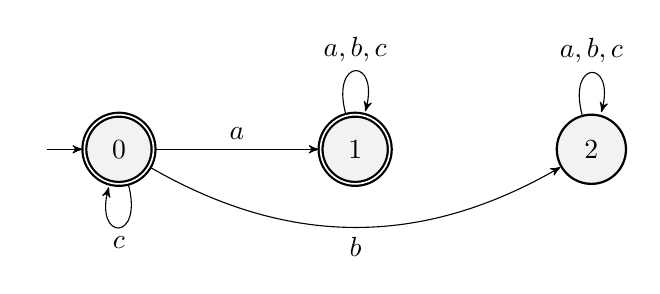
\begin{tikzpicture}
    \node[state, initial, accepting] (s0) {0};
    \node[state, right of=s0, accepting] (s1) {1};
    \node[state, right of=s1] (s2) {2};
    \draw (s0) edge[above] node{$a$} (s1);
    \draw (s0) edge[bend right, below ] node{$b$} (s2);
    \draw (s0) edge[loop below] node{$c$} (s0);
    \draw (s1) edge[loop above] node{$a,b,c$} (s1);
    \draw (s2) edge[loop above] node{$a,b,c$} (s2);
  \end{tikzpicture}
  \caption{2.1.a}
\end{figure}

\begin{figure}[p]
  \centering
  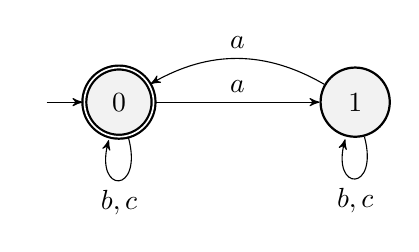
\begin{tikzpicture}
    \node[state, initial, accepting] (s0) {0};
    \node[state, right of=s0] (s1) {1};
    \draw (s0) edge[loop below] node{$b,c$} (s0);
    \draw (s0) edge[above] node{$a$} (s1);
    \draw (s1) edge[bend right, above] node{$a$} (s0);
    \draw (s1) edge[loop below] node{$b,c$} (s1);
  \end{tikzpicture}
  \caption{2.1.b}
\end{figure}

\begin{figure}[p]
  \centering
  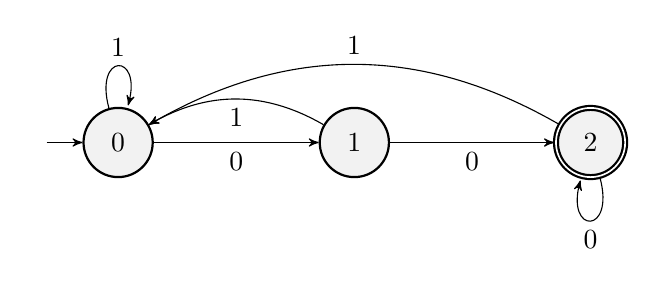
\begin{tikzpicture}
    \node[state, initial] (s0) {0};
    \node[state, right of=s0] (s1) {1};
    \node[state, right of=s1, accepting] (s2) {2};
    \draw (s0) edge[loop above] node{1} (s0);
    \draw (s0) edge[below] node{0} (s1);
    \draw (s1) edge[bend right, below] node{1} (s0);
    \draw (s1) edge[below] node{0} (s2);
    \draw (s2) edge[bend right, above] node{1} (s0);
    \draw (s2) edge[loop below] node{0} (s2);
  \end{tikzpicture}
  \caption{2.1.c}
\end{figure}

\begin{figure}[p]
  \centering
  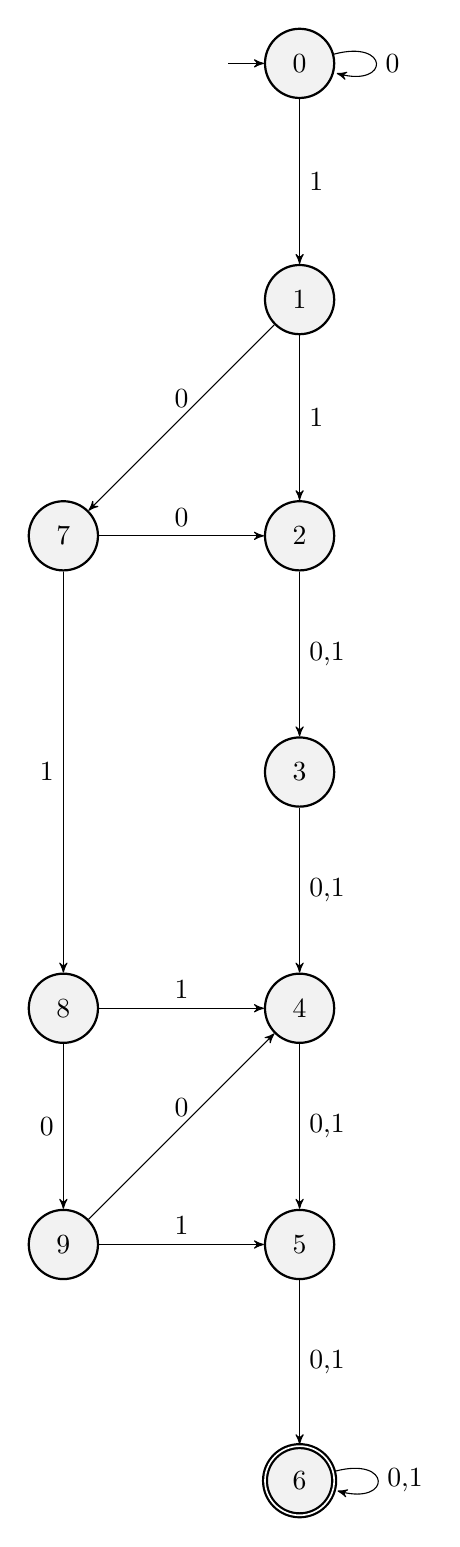
\begin{tikzpicture}
    \node[state, initial] (s0) {0};
    \node[state, below of=s0] (s1) {1};
    \node[state, below of=s1] (s2) {2};
    \node[state, below of=s2] (s3) {3};
    \node[state, below of=s3] (s4) {4};
    \node[state, below of=s4] (s5) {5};
    \node[state, below of=s5, accepting] (s6) {6};
    \node[state, left of=s2] (s7) {7};
    \node[state, left of=s4] (s8) {8};
    \node[state, left of=s5] (s9) {9};
    \draw (s0) edge[loop right] node{0} (s0);
    \draw (s0) edge[right] node{1} (s1);
    \draw (s1) edge[above] node{0} (s7);
    \draw (s1) edge[right] node{1} (s2);
    \draw (s2) edge[right] node{0,1} (s3);
    \draw (s3) edge[right] node{0,1} (s4);
    \draw (s4) edge[right] node{0,1} (s5);
    \draw (s5) edge[right] node{0,1} (s6);
    \draw (s6) edge[loop right] node{0,1} (s6);
    \draw (s7) edge[above] node{0} (s2);
    \draw (s7) edge[left] node{1} (s8);
    \draw (s8) edge[left] node{0} (s9);
    \draw (s8) edge[above] node{1} (s4);
    \draw (s9) edge[above] node{0} (s4);
    \draw (s9) edge[above] node{1} (s5);
  \end{tikzpicture}
  \caption{2.1.d}
\end{figure}

\begin{figure}[p]
  \centering
  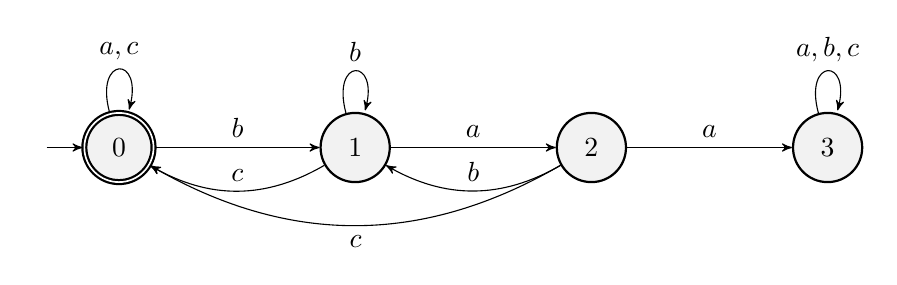
\begin{tikzpicture}
    \node[state, initial, accepting] (s0) {0};
    \node[state, right of=s0] (s1) {1};
    \node[state, right of=s1] (s2) {2};
    \node[state, right of=s2] (s3) {3};
    \draw (s0) edge[loop above] node{$a,c$} (s0);
    \draw (s0) edge[above] node{$b$} (s1);
    \draw (s1) edge[above] node{$a$} (s2);
    \draw (s1) edge[loop above] node{$b$} (s1);
    \draw (s1) edge[bend left, above] node{$c$} (s0);
    \draw (s2) edge[above] node{$a$} (s3);
    \draw (s2) edge[bend left, above] node{$b$} (s1);
    \draw (s2) edge[bend left, below] node{$c$} (s0);
    \draw (s3) edge[loop above] node{$a,b,c$} (s3);
  \end{tikzpicture}
  \caption{2.1.e}
\end{figure}

\begin{figure}[p]
  \centering
  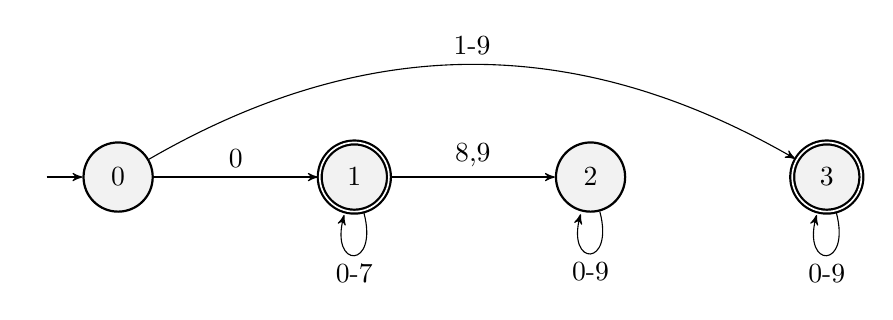
\begin{tikzpicture}
    \node[state, initial] (s0) {0};
    \node[state, right of=s0, accepting] (s1) {1};
    \node[state, right of=s1] (s2) {2};
    \node[state, right of=s2, accepting] (s3) {3};
    \draw (s0) edge[above] node{0} (s1);
    \draw (s0) edge[bend left, above] node{1-9} (s3);
    \draw (s1) edge[loop below] node{0-7} (s1);
    \draw (s1) edge[above] node{8,9} (s2);
    \draw (s2) edge[loop below] node{0-9} (s2);
    \draw (s3) edge[loop below] node{0-9} (s3);
  \end{tikzpicture}
  \caption{2.1.f}
\end{figure}

\begin{figure}[p]
  \centering
  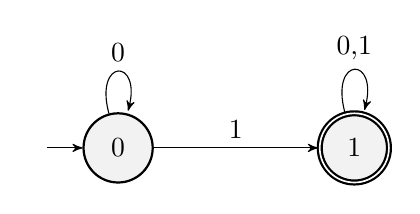
\begin{tikzpicture}
    \node[state, initial] (s0) {0};
    \node[state, right of=s0, accepting] (s1) {1};
    \draw (s0) edge[loop above] node{0} (s0);
    \draw (s0) edge[above] node{1} (s1);
    \draw (s1) edge[loop above] node{0,1} (s1);
  \end{tikzpicture}
  \caption{2.1.g. Since $a^n + b^n = c^n$ can have integer solutions and not just
    positive integer solutions when $n = 0$ then there are no solutions and when 
    $n > 0$ then $a = b = c = 0$ is always a solution. The goal is to construct
    a DFA that accepts the binary representations of all numbers greater than
    0.}
\end{figure}

\begin{figure}[p]
  \centering
  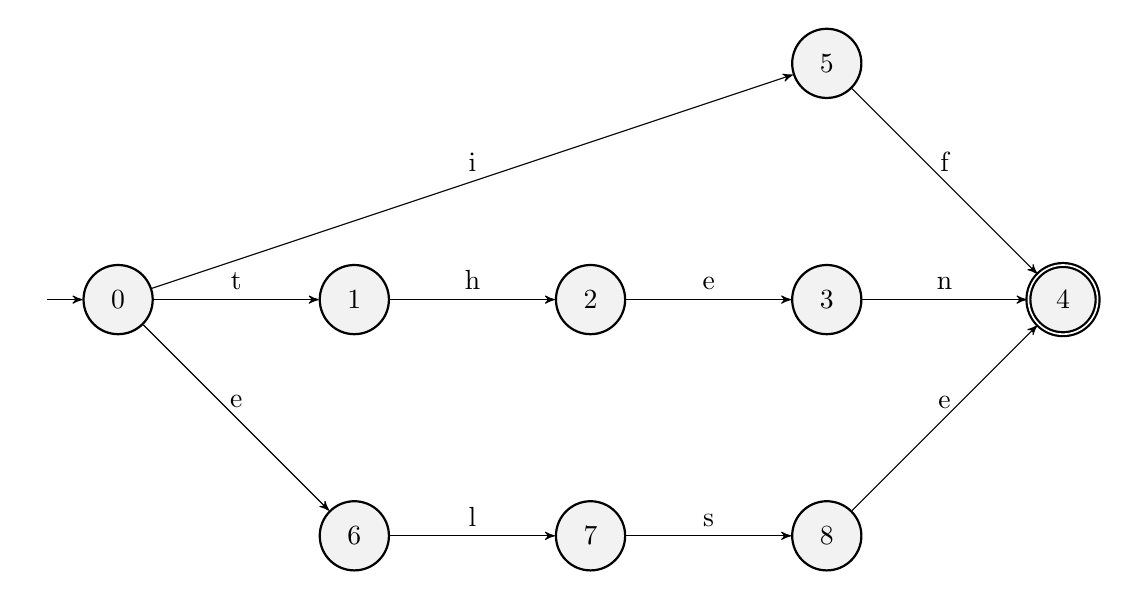
\begin{tikzpicture}
    \node[state, initial] (s0) {0};
    \node[state, right of=s0] (s1) {1};
    \node[state, right of=s1] (s2) {2};
    \node[state, right of=s2] (s3) {3};
    \node[state, right of=s3, accepting] (s4) {4};
    \node[state, above of=s3] (s5) {5};
    \node[state, below of=s1] (s6) {6};
    \node[state, below of=s2] (s7) {7};
    \node[state, below of=s3] (s8) {8};
    \draw (s0) edge[above] node{t} (s1);
    \draw (s1) edge[above] node{h} (s2);
    \draw (s2) edge[above] node{e} (s3);
    \draw (s3) edge[above] node{n} (s4);
    \draw (s0) edge[above] node{i} (s5);
    \draw (s5) edge[above] node{f} (s4);
    \draw (s0) edge[above] node{e} (s6);
    \draw (s6) edge[above] node{l} (s7);
    \draw (s7) edge[above] node{s} (s8);
    \draw (s8) edge[above] node{e} (s4);
  \end{tikzpicture}
  \caption{2.4.a}
\end{figure}

\begin{figure}[p]
  \centering
  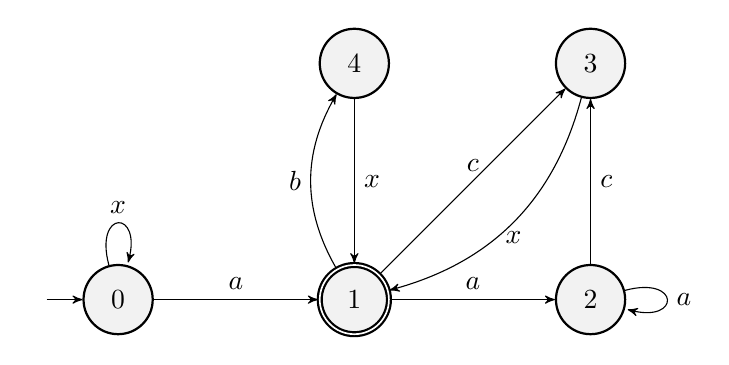
\begin{tikzpicture}
    \node[state, initial] (s0) {0};
    \node[state, right of=s0, accepting] (s1) {1};
    \node[state, right of=s1] (s2) {2};
    \node[state, above of=s2] (s3) {3};
    \node[state, left of=s3] (s4) {4};
    \draw (s0) edge[loop above] node{$x$} (s0);
    \draw (s0) edge[above] node{$a$} (s1);
    \draw (s1) edge[bend left, left] node{$b$} (s4);
    \draw (s1) edge[above] node{$a$} (s2);
    \draw (s1) edge[above] node{$c$} (s3);
    \draw (s2) edge[loop right] node{$a$} (s2);
    \draw (s2) edge[right] node{$c$} (s3);
    \draw (s3) edge[bend left, below] node{$x$} (s1);
    \draw (s4) edge[right] node{$x$} (s1);
  \end{tikzpicture}
  \caption{2.4.b}
\end{figure}

\begin{figure}[p]
  \centering
  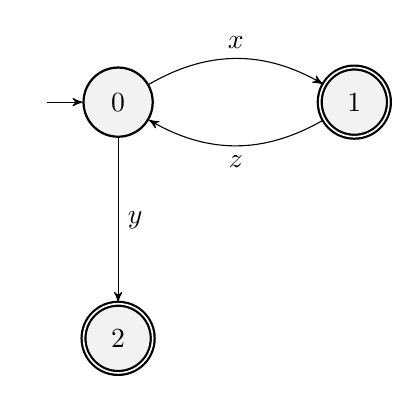
\begin{tikzpicture}
    \node[state, initial] (s0) {0};
    \node[state, right of=s0, accepting] (s1) {1};
    \node[state, below of=s0, accepting] (s2) {2};
    \draw (s0) edge[bend left, above] node{$x$} (s1);
    \draw (s0) edge[right] node{$y$} (s2);
    \draw (s1) edge[bend left, below] node{$z$} (s0);
  \end{tikzpicture}
  \caption{2.5.a} 
\end{figure}

\begin{figure}[p]
  \centering
  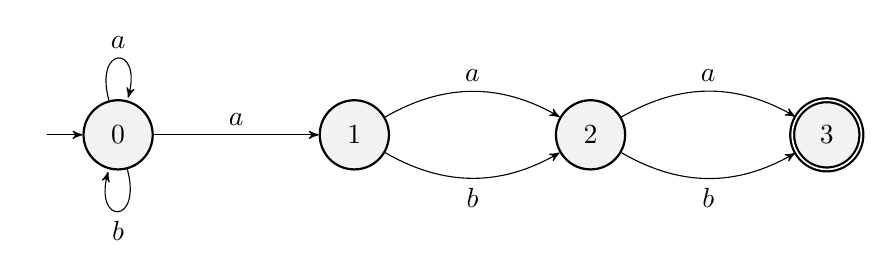
\begin{tikzpicture}
    \node[state, initial] (s0) {0};
    \node[state, right of=s0] (s1) {1};
    \node[state, right of=s1] (s2) {2};
    \node[state, right of=s2, accepting] (s3) {3};
    \draw (s0) edge[loop above] node{$a$} (s0);
    \draw (s0) edge[loop below] node{$b$} (s0);
    \draw (s0) edge[above] node{$a$} (s1);
    \draw (s1) edge[bend left, above] node{$a$} (s2);
    \draw (s1) edge[bend right, below] node{$b$} (s2);
    \draw (s2) edge[bend left, above] node{$a$} (s3);
    \draw (s2) edge[bend right, below] node{$b$} (s3);
  \end{tikzpicture}
  \caption{2.5.b. The original NFA accepts a string if and only if it is at
    least five symbols long and the fifth-from-last symbol is ``a''. This
    simpler NFA accepts a string if and only if it is at least three symbols
    long and the third-from-last symbol is ``a''.} 
\end{figure}

\begin{figure}[p]
  \centering
  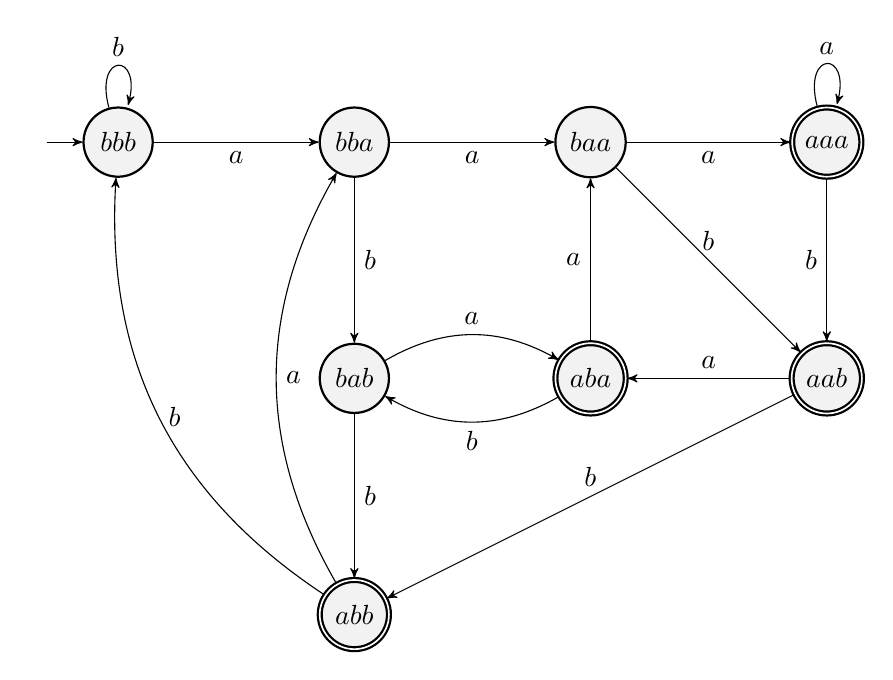
\begin{tikzpicture}
    \node[state, initial] (bbb) {$bbb$};
    \node[state, right of=bbb] (bba) {$bba$};
    \node[state, right of=bba] (baa) {$baa$};
    \node[state, right of=baa, accepting] (aaa) {$aaa$};
    \node[state, below of=bba] (bab) {$bab$};
    \node[state, right of=bab, accepting] (aba) {$aba$};
    \node[state, right of=aba, accepting] (aab) {$aab$};
    \node[state, below of=bab, accepting] (abb) {$abb$};

    \draw (bbb) edge[below] node{$a$} (bba);
    \draw (bbb) edge[loop above] node{$b$} (bbb);

    \draw (bba) edge[below] node{$a$} (baa);
    \draw (bba) edge[right] node{$b$} (bab);

    \draw (baa) edge[below] node{$a$} (aaa);
    \draw (baa) edge[above] node{$b$} (aab);

    \draw (aaa) edge[loop above] node{$a$} (aaa);
    \draw (aaa) edge[left] node{$b$} (aab);

    \draw (bab) edge[bend left, above] node{$a$} (aba);
    \draw (bab) edge[right] node{$b$} (abb);

    \draw (aba) edge[left] node{$a$} (baa);
    \draw (aba) edge[bend left, below] node{$b$} (bab);

    \draw (aab) edge[above] node{$a$} (aba);
    \draw (aab) edge[above] node{$b$} (abb);

    \draw (abb) edge[bend left, right] node{$a$} (bba);
    \draw (abb) edge[bend left, right] node{$b$} (bbb);
  \end{tikzpicture}
  \caption{2.5.b. It really helps to remember that since the DFA only has to
    ``keep track of'' just the last three characters seen and as there are just
    two characters in the alphabet then having $2^3$ states is enough.
    Additionally the strategy is that if we're at the state for words where the
    last three characters is $xyz$ where $x, y, z \in \{a, b\}$ then upon seeing
    an $a$ the automaton should transition to the state for words where the last
    three characters are $yza$. Finally any state of the form $axy$ is an
    accepting state.}
\end{figure}

\begin{figure}[p]
  \centering
  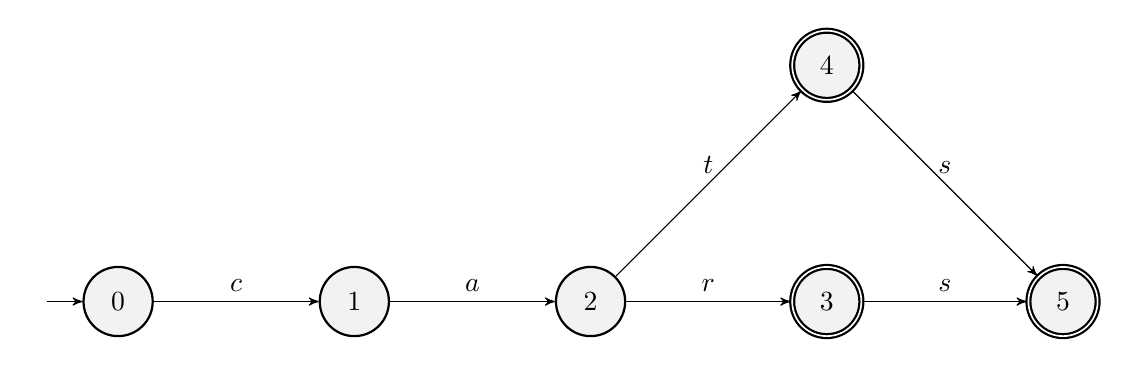
\begin{tikzpicture}
    \node[state, initial] (s0) {0};
    \node[state, right of=s0] (s1) {1};
    \node[state, right of=s1] (s2) {2};
    \node[state, right of=s2, accepting] (s4) {3};
    \node[state, above of=s4, accepting] (s3) {4};
    \node[state, right of=s4, accepting] (s5) {5};

    \draw (s0) edge[above] node{$c$} (s1);
    \draw (s1) edge[above] node{$a$} (s2);
    \draw (s2) edge[above] node{$t$} (s3);
    \draw (s2) edge[above] node{$r$} (s4);
    \draw (s3) edge[above] node{$s$} (s5);
    \draw (s4) edge[above] node{$s$} (s5);
  \end{tikzpicture}
  \caption{2.5.c}
\end{figure}

\begin{figure}[p]
  \centering
  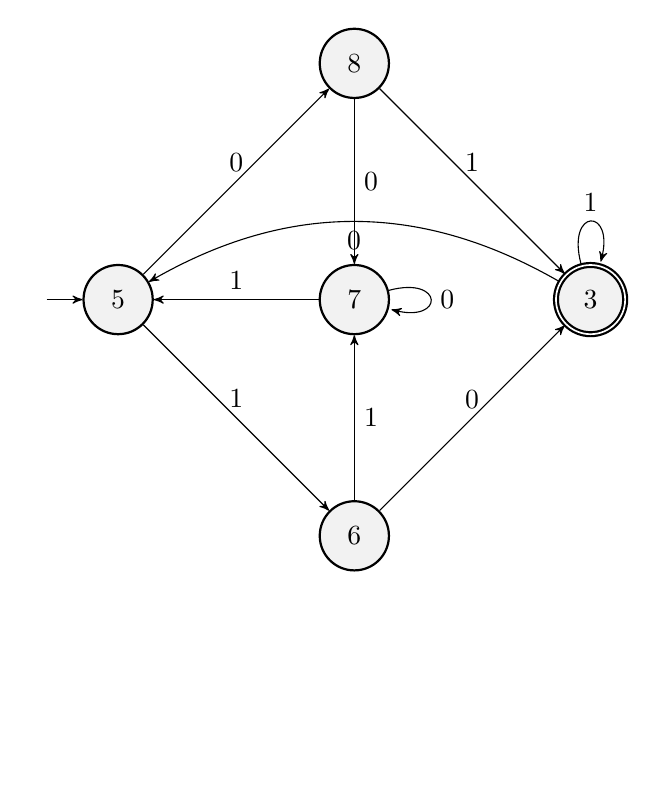
\begin{tikzpicture}
    \node[state, initial]                (s5) {5};
    \node[state, right of=s5]            (s7) {7};
    \node[state, below of=s7]            (s6) {6};
    \node[below of=s6]                   (e)  {};
    \node[state, above of=s7]            (s8) {8};
    \node[state, right of=s7, accepting] (s3) {3};

    \draw (s5) edge[above] node{0} (s8);
    \draw (s5) edge[above] node{1} (s6);
    \draw (s7) edge[loop right] node{0} (s7);
    \draw (s7) edge[above] node{1} (s5);
    \draw (s6) edge[above] node{0} (s3);
    \draw (s6) edge[right] node{1} (s7);
    \draw (s8) edge[right] node{0} (s7);
    \draw (s8) edge[above] node{1} (s3);
    \draw (s3) edge[bend right, below] node{0} (s5);
    \draw (s3) edge[loop above] node{1} (s3);
  \end{tikzpicture}
  \caption{2.6}
\end{figure}


\end{document}
